%% DONE
\id{ҒТАМР 65.33.29}{https://doi.org/10.58805/kazutb.v.1.26-833}

\begin{articleheader}
\sectionwithauthors{Д.Қ. Алибаев, А.Ж. Иманбаев, Hulya Gul, Г.Е. Есиркеп, Ж. Нармандах}{АСҚАБАҚ ҚҰРАМДАС БӨЛІКТЕРІНЕН ТҰТАС ДӘНДІ БИДАЙ ҰНЫНАН ЖАСАЛҒАН ҚЫТЫРЛАҚ НАН. Бөлім 1. ВИТАМИНДІК ҚҰРАМЫ МЕН МИКРОБИОЛОГИЯЛЫҚ ЗЕРТТЕУЛЕРІ}

{\bfseries 
\textsuperscript{1}Д.Қ. Алибаев\textsuperscript{\envelope } \authorid,
\textsuperscript{1}А.Ж. Иманбаев\authorid,
\textsuperscript{2}Hulya Gul\authorid,
\textsuperscript{3}Г.Е. Есиркеп\authorid,
\textsuperscript{3}Ж. Нармандах\authorid}
\end{articleheader}

\begin{affiliation}
\emph{\textsuperscript{1}М.Әуезов атындағы Оңтүстік Қазақстан университеті, Шымкент,Қазақстан,}

\emph{\textsuperscript{2}Сулеймен Демирел Универсиетті, Испарта, Турция,}

\emph{\textsuperscript{3}Қ.Құлажанов атындағы Қазақ технология және бизнес университеті, Астана, Қазақстан,}

\textsuperscript{\envelope }{\em Корреспондент-автор: dinaalibayeva3@gmail.com}
\end{affiliation}

Бұл мақалада асқабақ дәні мен қабығы қосылған тұтас дәнді бидай ұнынан
жасалған қытырлақ нанның витаминдік құрамы, денсаулыққа пайдасы және
микробиологиялық қасиеттері зерттеледі. Асқабақтың құрамындағы маңызды
қоректік заттар, оның ішінде дәрумендер мен минералдар, иммундық жүйені
нығайтуға және ас қорыту жүйесінің жұмысын жақсартуға әсер етеді. Тұтас
дәнді бидай ұнының жоғары талшықты құрамы қытырлақ нан (хлебцыдің)
қоректік құндылығын арттырады, сонымен қатар микробиологиялық зерттеулер
нәтижесінде өнімнің тағамдық қауіпсіздігі мен тұрақтылығы бағаланады.

Зерттеу барысында қытырлақ нанның химиялық құрамы талданып, оның
витаминдік құрамы анықталды. Сонымен қатар, дайын өнімнің
микробиологиялық қауіпсіздігі бағаланып, патогенді микроорганизмдердің
болуына талдау жасалды. Нәтижелер асқабақ дәні мен қабығы қосылған
қытырлақ нан құрамында β-каротин мен витаминдердің мөлшері жоғары
деңгейлері бар екенін көрсетті. Сонымен қатар, өнімдернің
микробиологиялық көрсеткіштері санитарлық-гигиеналық нормаларға сәйкес
келетіндігі анықталды.

Мақалада мақсаты асқабақ қабығы мен дәнімен байытылған бүтін бидай
ұнынан жасалған қытырлақ нанның құрамындағы витаминдердің құрамы және
микробиологиялық зерттеу нәтижелерін ұсыну және талқылау. Адам
денсаулығына пайдасын түсіндіру, оның құрамындағы витаминдердің
артықшылықтарын атап өту арқылы оқырмандарды салауатты және қолжетімді
тамақтануға ынталандыру.

Осылайша, асқабақ қабығы мен дәні қосылған тұтас дәнді бидай ұнынан
жасалған қытырлақ нан функционалды тағамдық өнім ретінде қарастырылады
және тұтынушыларға денсаулыққа пайдалы балама ретінде ұсынылуы мүмкін.

Түйін сөздер: асқабақ дәні, асқабақ қабығы, тұтас дәнді бидай ұны,
қытырлақ нан, дәрумендер, микробиологиялық көрсеткіштер.

\begin{articleheader}
{\bfseries ХРУСТЯЩИЙ ХЛЕБ ИЗ ЦЕЛЬНОПШЕНИЧНОЙ МУКИ С ЧАСТИКАМИ ТЫКВЫ. Часть 1. ВИТАМИННЫЙ СОСТАВ И МИКРОБИОЛОГИЧЕСКИЕ ИССЛЕДОВАНИЯ}

{\bfseries
\textsuperscript{1}Д.К. Алибаева\textsuperscript{\envelope },
\textsuperscript{1}А.Ж. Иманбаев,
\textsuperscript{2}Hulya Gul,
\textsuperscript{3}Г.Е. Есиркеп,
\textsuperscript{3}Ж. Нармандах}
\end{articleheader}

\begin{affiliation}
\emph{\textsuperscript{1}Южно-Казахстанский университет им. М. Ауэзова, Шымкент, Казахстан,}

\emph{\textsuperscript{2}Сулеймен Демирель Университет, Испарта, Турция,}

\emph{\textsuperscript{3}Казахский университет технологии и бизнеса имени К.Кулажанова, Астана, Казахстан,}

e-mail:\href{mailto:dinaalibayeva3@gmail.com}{\nolinkurl{dinaalibayeva3@gmail.com}}
\end{affiliation}

В этой статье исследуется витаминный состав, польза для здоровья и
микробиологические свойства хлебца из цельнозерновой пшеничной муки с
добавлением тыквенных семечек и кожуры. Важные питательные вещества,
содержащиеся в тыкве, в том числе витамины и минералы, способствуют
укреплению иммунной системы и улучшению работы пищеварительной системы.
Высокое содержание клетчатки в цельнозерновой пшеничной муке повышает
питательную ценность хрустящего хлеба (хлебца), а также в результате
микробиологических исследований оценивается пищевая безопасность и
стабильность продукта.

В ходе исследования был проанализирован химический состав хрустящего
хлеба и определен его витаминный состав. Кроме того, была проведена
оценка микробиологической безопасности готовой продукции и проведен
анализ на наличие патогенных микроорганизмов. Результаты показали, что
хрустящий хлеб с тыквенными семечками и кожурой содержит высокий уровень
β-каротина и витаминов. Кроме того, установлено, что микробиологические
показатели продукции соответствуют санитарно-гигиеническим нормам.

В статье цель состоит в том, чтобы представить и обсудить содержание
витаминов в хрустящем хлебе из цельной пшеничной муки, обогащенной
кожурой и зернами тыквы, а также результаты микробиологических
исследований. Объясняя пользу для здоровья человека и подчеркивая
преимущества витаминов в составе, побудить читателей к здоровому и
доступному питанию.

Таким образом, хрустящий хлеб из цельнозерновой пшеничной муки с
тыквенной кожурой и зернами считается функциональным пищевым продуктом и
может быть предложен потребителям в качестве более здоровой
альтернативы.

{\bfseries Ключевые слова:} тыквенные семечки, тыквенная кожура,
цельнозерновая пшеничная мука, хрустящий хлеб, витамины,
микробиологические показатели.

\begin{articleheader}
{\bfseries CRISPY BREAD MADE WITH WHOLE WHEAT FLOUR WITH PUMPKIN PARTS. Part 1. VITAMIN COMPOSITION AND MICROBIOLOGICAL STUDIES}

{\bfseries
\textsuperscript{1}D.K. Alibayeva\textsuperscript{\envelope },
\textsuperscript{1}A.Zh. Imanbayev,
\textsuperscript{2}Hulya Gul,
\textsuperscript{3}G.E. Esirkep,
\textsuperscript{3}Zh. Narmandakh}
\end{articleheader}

\begin{affiliation}
\emph{\textsuperscript{1}South Kazakhstan University named after M. Auezov, Shymkent, Kazakhstan,}

\emph{\textsuperscript{2}Suleyman Demirel University, Isparta, Turkey,}

\emph{\textsuperscript{3}Kazakh University of Technology and Business named after K.Kulazhanov, Astana, Kazakhstan,}

e-mail: dinaalibayeva3@gmail.com
\end{affiliation}

This article examines the vitamin composition, health benefits and
microbiological properties of whole grain wheat flour crispbread with
the addition of pumpkin seeds and peel. The important nutrients
contained in pumpkin, including vitamins and minerals, have the effect
of strengthening the immune system and improving the functioning of the
digestive system. The high fiber content of whole grain wheat flour
increases the nutritional value of crispbread (khlebtsy), as well as the
nutritional safety and stability of the product are assessed as a result
of microbiological studies.

In the course of the study, the chemical composition of crispbread was
analyzed and its vitamin composition was determined. In addition, the
microbiological safety of the finished product was evaluated and an
analysis was made for the presence of pathogenic microorganisms. The
results showed that crispbread with pumpkin seeds and peel contains high
levels of β-carotene and vitamins. In addition, it was found that the
microbiological indicators of the products correspond to sanitary and
hygienic standards.

The article aims to present and discuss the content of vitamins in whole
wheat flour crispbread enriched with pumpkin peel and seeds and the
results of microbiological research. Encourage readers to eat healthy
and affordable by explaining the benefits to human health, highlighting
the benefits of the vitamins it contains.

Thus, crispbread made from whole grain wheat flour with pumpkin peel and
seeds is considered as a functional food product and can be offered to
consumers as a healthier alternative.

{\bfseries Keywords:} pumpkin seed, pumpkin peel, whole grain wheat flour,
crispbread, vitamins, microbiological indicators.

\begin{multicols}{2}
{\bfseries Кіріспе.} Қазіргі таңда дұрыс тамақтану мен денсаулықты
сақтау мәселелері әлем бойынша үлкен мәнге ие болып отыр. Әсіресе,
табиғи және қоректік қасиеттері жоғары өнімдерге деген сұраныс артуда.
Тұтас дәнді бидай ұны мен асқабақтың құрамдас бөліктерін пайдалану
арқылы дайындалған тағамдар осындай трендті толықтай қанағаттандырады.
Бұл өнімдер жоғары қоректік құндылыққа ие, себебі асқабақ дәні мен
қабығының құрамында витаминдер, минералдар, антиоксиданттар және басқа
да пайдалы заттар бар. Тұтас дәнді бидай ұнының талшықты құрамының көп
болуы, оның ас қорыту жүйесін жақсартуға, қант деңгейін тұрақтандыруға
және жүрек-қан тамырлары жүйесінің жұмысын қолдауға ықпалы бар {[}1{]}.

Асқабақ - бұл дәстүрлі түрде пайдалы тағам ретінде қолданылып келген
көкөніс, оның дәндері мен қабығы да денсаулыққа зор пайда әкелетіні
белгілі. Асқабақтың құрамындағы магний, калий, темір, және селен сияқты
минералдар ағзаның иммундық жүйесін нығайтып, күйзелістен қорғайды.
Сонымен қатар, оның құрамында дәрумендер (әсіресе, А дәрумені) мен
антиоксиданттар қабынуға қарсы әсер көрсетіп, қартаю үдерісін
баяулатады. Бұдан басқа, асқабақтың талшықты құрамы ас қорыту жүйесін
реттеп, ішектің микробиологиялық теңгерімін жақсартады {[}2{]}.

Тұтас дәнді бидай ұнының ерекше қасиеттері оның құрамындағы қоректік
заттардың толық сақталуында жатыр. Тұтас дәнді бидай талшыққа,
витаминдер мен минералдарға бай болғандықтан, олар ағзаға қажетті
қоректік заттарды толықтай қамтамасыз етеді. Тұтас дәнді бидай ұнының
көмірсулары баяу қорытылады, бұл қандағы қант деңгейінің күрт өзгеруіне
жол бермей, ұзақ уақыт бойы энергия береді {[}3{]}.

Бұл мақалада асқабақ дәні мен қабығы қосылған тұтас дәнді бидай ұнынан
жасалған қытырлақ нан (хлебцыдің) витаминдік құрамы, денсаулыққа пайдасы
және микробиологиялық көрсеткіштері зерттеледі. Атап айтқанда, асқабақ
пен тұтас дәнді бидай ұнының бірігуі бұл өнімнің қоректік құндылығын
арттырып, оның тағамдық маңыздылығын ерекше етеді. Сонымен қатар,
өнімнің микробиологиялық зерттеулері оның тағамдық қауіпсіздігі мен ұзақ
мерзімді сақталуының тиімділігін бағалауға мүмкіндік береді {[}4{]}.

Зерттеу барысында асқабақ пен тұтас дәнді бидай ұнынан жасалған қытырлақ
нан (хлебцыдің) ағзаға әсері, олардың құрамындағы пайдалы заттардың
тағамдық құндылығы және микробиологиялық қауіпсіздігі туралы ғылыми
деректер жинақталды. Бұл өнімдердің салауатты өмір салтын ұстанушы
адамдар үшін маңыздылығы мен олардың денсаулыққа оң әсер етуі туралы
қорытынды жасалады. Мақала сонымен қатар, асқабақ және тұтас дәнді бидай
ұнының денсаулыққа пайдалы әсерлерін көрсететін жаңадан алынған
деректерді ұсынады {[}5{]}.

\href{https://www.sciencedirect.com/topics/biochemistry-genetics-and-molecular-biology/healthy-lifestyle}{Қазіргі
уақытта тұтынушылардың салауатты өмір салтын} насихаттайтын денсаулыққа
бағытталған азық-түлік туралы деректер артты. Тұтынушылар адам
денсаулығына оң әсерін тигізетін, оңай дайындалатын және тағамдық
құндылығы жоғары тағамдарға қол жеткізуге құштар. Бұл салауатты
азық-түлік өнімдеріне деген құштарлық жылдар бойы өсуде {[}6{]}.

Асқабақ - ең жиі тұтынылатын көкөністердің бірі. Сонымен қатар қоректік,
емдік, және экономикалық пайдасы зор. Асқабақтың калориясы төмен, бірақ
А дәрумені, С дәрумені, калий және талшық секілді маңызды қоректік
заттар көп. Асқабақтың етті бөлігі тұтынуға пайдаланылады, ал жалпы
жемістің шамамен 18-21\% қалдық ретінде қалады {[}7{]}.

Қалдықтарды тиімді пайдалану - қазіргі таңда маңызды мәселелердің бірі.
Асқабақтың қабығы, тұқымдары және гүлдері мен жапырақтары жоғары құнды
өнімге айналуы мүмкін, себебі, биоактивті қосылыстардың бай көзі болып
табылады. Бірақ тағамдық пайдасы бар биоактивті химиялық заттардың бай
көзі болғанына қарамастан асқабақ тұқымдары мен қабықтары жиі қалдық
ретінде саналады. Үндістанның кейбір бөліктерінде асқабақтың қабығы,
жапырақтары мен гүлдері тамақ ретінде сирек жейді. Асқабақтың фракциялық
құрамы 10-12\% қабығы 3-4\% целлюлоза, 79-82\% еті және 4-6\% тұқымдық
асқабақ ұнын қолданатын кеңейтілген тағамдарды әзірлеу бойынша зерттеуде
жіктелген {[}8,9{]}.

Тұтас дәнді бидай ұнының кебек, ұрық және эндеспермда адам ағзасына
қажетті көптеген микроэлементтер мен дәрумендерді қамтиды. Кебектегі ең
құнды зат, ол тағамдық талшық -- жасұнық. Ол ең маңызды бола тұра, адам
ағзасында мүлдем сіңбейді және асқазан мен ішек жолдары үшін тазалағыш
ретінде ағзадан толығымен шығып кетеді. Ондағы қожды, токсиндерді, ауыр
металдарды және олардың тұздарын ағзадан оңай шығарады. Дегенмен,
кебектегі минералды элементтер, дәрумендер және ферменттер ағзамен оңай
сіңіріледі {[}10,11{]}.

Тұтас дәнді бидай ұнынан дайындалған нан өнімдері тамақтану мәзірінде
ерекше орын алады, себебі олар жоғары қоректік құндылыққа ие. Сондықтан
да қазіргі уақытта тамақ өнеркәсібі тұтас дәнді бидай ұнын енгізу арқылы
аспаздық өнімдерінің жаңа түрлерін игеруге үлкен көңіл бөлуде
{[}12,13{]}.

Осындай екі маңызды ингредиентті біріктіріп, біз қытырлақ нан (хлебцы)
рецептурасын әзірлеуді ұсынамыз. Бұл өнім тек дәмді ғана емес, сонымен
қатар денсаулыққа пайдалы. Асқабақ дәні мен қабығы қосылған тұтас дәнді
бидай ұнынан жасалған қытырлақ нанның А, Е, С, В тобы және β - каротин
витаминдерге бай екені төменде дәлелденді {[}14,15{]}.

А, Е, С, В тобы және β - каротин витаминдерді анықтау үшін сұйықтықты
хроматография (HPLC) - өте сезімтал және дәл әдіс, ол көптеген
биологиялық және химиялық заттарды, соның ішінде дәрумендерді анықтау
үшін кеңінен қолданылады. Бұл әдіс арқылы дәрумендер жиынтығын талдауға
болады, оларды бөлу және анықтау үшін арнайы хроматографиялық
колонкалар, еріткіштер мен детекторлар пайдаланылады {[}16,17{]}.

HPLC әдісінің негізгі принципі - қоспаларды (және дәрумендерді)
еріткіштің әсерінен хроматографиялық колонка арқылы ажырату. Әрбір
дәруменнің бөлек физикалық-химиялық қасиеттері, оның ішінде полярлығы
мен молекулалық салмағы болады, сондықтан олар колонка арқылы әртүрлі
жылдамдықпен өтеді және әрқайсысының шығу уақыты әртүрлі болады.
Нәтижесінде, әр дәруменді жеке-жеке анықтауға болады {[}17,18{]}.

КМАФАнМ - жалпы микроорганизмдер санын анықтайды, тағамның
микробиологиялық сапасын бағалауға көмектеседі. БГКП -- патогенді
бактериялардың, әсіресе тамақтан улану мен аурулар тудыратын
микроорганизмдердің санын анықтайды. Плесеньдер -- тағамдағы сақталу
жағдайының дұрыстығын және микробиологиялық сапаны бақылауға арналған
{[}19{]}.

{\bfseries Материалдар мен әдістер.} Бұл зерттеу асқабақ дәні мен қабығы
қосылған тұтас дәнді бидай ұнынан жасалған қытырлақ нанның А, Е, С, В
тобы және β-каротин витаминдерді және микробиологиялық көрсеткіштерін
Алматы Технологиялық Университетінің Техникалық реттеу және метрология
комитетінің Ұлттық аккредиттеу орталығының шешімімен «Тағам
қауіпсіздігі» сынақ зертханасы «Сынақ және калибрлеу зертханаларының
құзыреттілігіне қойылатын жалпы талаптар» МЕМСТ ИСО/IEC 17025-2019
талаптарына сәйкес Қазақстан Республикасының аккредиттеу жүйесінде
аккредиттелген (аккредиттеу аттестаты № KZ.T.02.E 1158 ) зертхана
орталығында жасалды.

Бақылау үлгісі ретінде алынған асқабақ дәні мен қабығы қосылған тұтас
дәнді бидай ұнынан жасалған қытырлақ нанның А, Е, С, В тобы және
β-каротин витаминдердің мөлшері дәлдікпен анықтау үшін сұйық
хроматографияның (ВЭЖХ/HPLC) әдісімен анықталды. Эксперимент
нәтижелерінің төменде 2-3 суретте мақалада келтірілген.

Асқабақ дәні мен қабығы қосылған тұтас дәнді бидай ұнынан жасалған
қытырлақ нанның құрамындағы А, Е және β-каротин витаминдерді талдаймыз.
10 г үлгі ұнтағына 1 г
~C\textsubscript{6}H\textsubscript{6}O\textsubscript{3}, 70 мл
C\textsubscript{2}H\textsubscript{5}OH және 30 мл (50\%) KOH қосылды,
араластырылды және 50 ± 2°c температурада су ваннасы арқылы 40 минут
бойы рефлюксацияланды. Сығындыны бейтараптандыру үшін қос дистилденген
су пайдаланылды, ол сусыз Na₂SO₄ көмегімен сусыздандырылды. Сонымен
қатар, сығынды су ваннасын (50 ± 2°c) қолдану арқылы шамамен 5 мл-ге
дейін концентрацияланды, метанолды қолдану арқылы 10 мл-ге дейін
сұйылтылды, 0,45 мкм мембрана арқылы сүзілді және соңында HPLC талдауына
ұшырады. RP-HPLC талдауы диодты массив детекторын Agilent 1100 сериялы
HPLC жүйесімен жүргізілді. β -каротиннің мөлшерін анықтау үшін CH₃CN (88
: 10 : 2) еріткіші бар Agilent tc-C18. Бағанасы (5 мкм, 4,6 × 250 мм).
Пайдаланылды және ультракүлгін сәулелердің сіңуі 453 нм-де тіркелді.
Майда еритін витаминдер үшін Agilent Eclipse XDB-C18 бағанасы қолданылды
(5 мкм, 4. 6 × 150 мм), еріткіш метанол болды және ультракүлгін
сәулеленуді анықтау А дәрумені үшін 325 нм, Е дәрумені үшін 290 нм
тіркелді. Барлық витаминдердің бөлінуі изократиялық элюцияға негізделді
және еріткіштің шығыны 1 мл/мин деңгейінде сақталды.

С витамині анықтау үшін үлгіні ұнтақтап, оның 10 г араластырылып,
құрамында метафосфор қышқылы 0,3 М және CH₃COOH 1,4 М бар экстрактивті
ерітіндімен гомогенизацияланды. Қоспа конустық колбаға салынып, 10 000
айн / мин жылдамдықпен 15 минут араластырылды. Содан кейін қоспаны сүзгі
арқылы сүземіз. C₆H₈O₆ стандарты 100 мг С витамин HPO₃ (0,3 М)/
CH\textsubscript{3}COOH (1,4 М) ерітіндісінде 0,1 мг/мл соңғы
концентрацияда еріту арқылы дайындалды. Калибрлеу сызығы өлшенген
концентрацияның төрт деңгейіне негізделген сызықтық диапазонға
ауыстырылды. С витамині мөлшерін анықтау Agilent HPLC жүйесінде
жүргізілді. Хроматографиялық бөлінуге rp-HPLC бағанында жылжымалы фазаны
изократиялық жеткізу арқылы қол жеткізілді (A/B 33/67; A: 0,1 М
CH\textsubscript{3}COOK, рн = 4,9, B: CH3CN: су {[}50 : 50{]}) ағын
жылдамдығы 1 мл/мин. ультракүлгін сәулелердің сіңуі бөлме
температурасында 254 нм-де тіркелді.

В дәрумені тобы үлгіні ұнтақтап, оны 2 г 25 мл H2SO4 (0,1 Н)
ерітіндісіне салынып, 121°c температурада 30 минут бойы инкубацияланды.
Содан кейін салқындатылып, 2,5 М NaOAc рн 4,5-ке дейін реттелді және 50
мг Такадиастаза ферменті қосылды. Сүзгі арқылы сүзіп, фильтратты 50 мл
таза сумен сұйылтып, қайтадан микрокеуекті сүзгі (0,45 мкм) арқылы
сүзді. HPLC жүйесіне жиырма микролитр фильтрат енгізілді. В дәруменінің
мөлшерін анықтау в дәрумені стандарттарымен салыстыру арқылы жүзеге
асырылды. Тиамин, рибофлавин, ниацин, пиридоксин және кобаламинге
арналған стандартты ерітінділер бұрын хабарланғандай дайындалды {[}11,
12{]}. Хроматографиялық бөлінуге кері фазалық- (RP-) HPLC бағанында
(Agilent Zorbax Eclipse Plus C18; 250 × 4,6 мм i.d., 5 мкм) изократиялық
жеткізудің жылжымалы фазасы арқылы қол жеткізілді (A/B 33/67; A: MeOH,
B: 0,023 М H3PO4, рн = 3,54) 0,5 мл/мин жылдамдықпен. Ультракүлгін (УК)
сіңіру бөлме температурасында 270 нм-де тіркелді.

КМАФАнМ анықтау үшін үлгіні үнтақтап аламыз. Пальцер сұйытылған агарына
1 г себіледі. Содан кейін егу термостатқа орналастырылады. Мезофильді
микроорганизмдердің өсіру температурасы +37 \textsuperscript{0}С
құрайды. Термостатта 48 сағатқа инкубацияланады, содан кейін колониялар
саналады. Колониялардың әртүрлілігі мен олардың морфологиясы зерттеледі,
одан әрі талдау үшін кейбір микроорганизмдер анықталады. Нәтижесінде
КМАФАнМ саны колониялар санына негізделіп, әрбір миллилитр немесе грамм
үшін есептеледі. Осылайша, өнімнің микробиологиялық сапасы анықталады.

БГКП анықтау үшін үлгіні Эндо агар қоректік ортаға себу арқылы зерттеу
жүргізіледі. Содан кейін егу термостатқа орналастырылады. Инкубациялада
температурасы 35°C, уақыты 48 сағат сақтаймыз. Колониялар морфологиясын
тексереді. БГКП үшін позитивті нәтижелер ерекше көкшіл түсті
ерекшеліктері бар колониялармен көрінеді. Егер патогенді кокк тәрізді
бактериялар табылса, өнімнің қауіпсіздігі мен сақталу мерзімі қайта
қаралады.

Плесеньдер анықтау үшін үлгісін стерильді ерітіндімен сұйылтып, Сабуро
агарын қоректік ортаға себіледі. Содан кейін егу термостатқа
орналастырылады. Инкубациялау температурасы 25-30°C, уақыты 3-7 күн.
Плесеньдердің колониялары дақтарды немесе дақ тәрізді құрылымдарды
көрсетеді. Инкубациядан кейін колониялар саны есептеледі және
микроскоппен тексеріледі. Нәтижесінде плесеньдердің саны колониялар
санына негізделіп есептеледі.

{\bfseries Нәтижелер мен талқылау.} Бұл рецепт асқабақ дәндері мен қабығын
пайдаланып, дәмді әрі пайдалы қытырлақ нан жасау үшін өте жақсы тәсіл.
Мына қадамдарды талдай отырып, әрбір кезеңнің маңыздылығына тоқталып
өтейік. Асқабақ қабығын жақсылап жуып, кептіріп аламыз.

Асқабақ қабығын жақсылап жуу оны сыртқы ластанудан тазартуға
көмектеседі. Содан кейін, кепкен асқабақ қабығымызды блендер көмегімен
ұсақтап аламыз. Асқабақ дәнін алдын ала қуырылады. Асқабақ дәнін қуыру
үшін, дәндерін қабығынан ажыратып, таза сумен жуып, құрғатыңыз. Содан
соң, пеште 180 \textsuperscript{0} С градус температурада 10 минут
қыздырамыз. Асқабақ дәндерін қуыру олардың хош иісін арттырады және
қытырлақтығын береді. Сонымен қатар, қуырылған дәндер нанның құрамына
қосымша дәм мен текстура қосады. Араластырғыш ыдысқа тұтас дәнді бидай
ұнын, асқабақ дәндерін, асқабақ қабығын және тұзды қосамыз. Барлық
құрғақ ингреденттерді жақсылап араластырамыз. Тұтас дәнді бидай ұнының
қосылуы нанда дәнді талшықтардың көп болуына және пайдалы болуына
мүмкіндік береді. Асқабақ қабығы мен дәндері басқа ингредиенттермен
жақсы араласқанда, нанның құрамында табиғи пайдалы заттар сақталады. Су
мен зәйтүн майын қосып, қамырды илейміз. Ашымалымыздың консистенциясы
жұмсақ, бірақ қолға жабыспайтын болуы қажет. Ашымалыны 5-15 минутқа
қалдырамыз. Пешімізді 180ºС температурада қыздырамыз. Табамызға
ашымалыны жұқа етіп жайып, пешімізге саламыз. 15 минуттан соң, пештен
алып, пышақпен кесіп формаға келтіреміз. Нанымызды қайта пешке 20-25
минутқа қалдырамыз. Піскен соң қытырлақ нанымызды салқындатамыз.
Салқындағаннан кейін, қытырлақ болуы үшін 5 минуттай қалдырамыз.
Тағамдық және биологиялық құндылығын жақсарту үшін қытырлақ нан (хлебцы)
нанына 15-45\% асқабақ қабығы мен дәнін ұнтақтап қосылды. Жүргізілген
зерттеулер нәтижесінде оңтайлы нұсқасы болып 30\% асқабақ қабығы мен
дәнін қосылған диеталық хлебцы өнімін алудың әдісі таңдалды. Төменде
1-суретте көруімізге болады.
\end{multicols}

\begin{figure}[H]
	\centering
	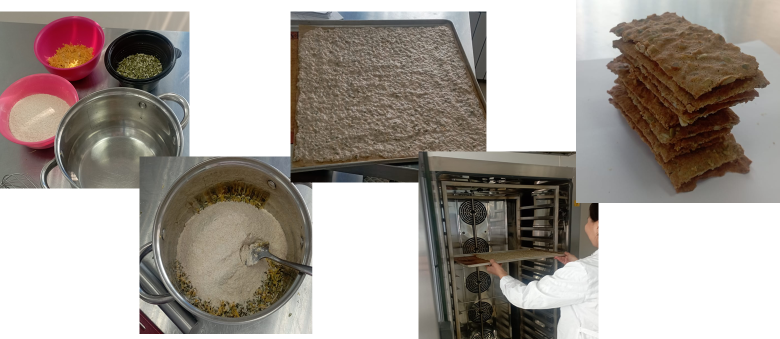
\includegraphics[width=0.8\textwidth]{media/pish2/image4}
	\caption*{1 - сурет. Байытылған қытырлақ нан жасау әдісі}
\end{figure}

\begin{multicols}{2}
Барлық дәрумендер HPLC әдісі арқылы анықталды, ол жоғары сезімталдық пен
дәлдікпен дәрумендердің нақты концентрациясын өлшеуге мүмкіндік берді.
Алынған деректердің қайталанғыштығы жоғары болды, нәтижесінде бұл әдіс
дәрумендердің салыстырмалы түрде төмен концентрацияларын дәл анықтауға
мүмкіндік берді.

Зерттеу барысында А, В, С, Е дәрумендерінің концентрациялары асқабақтың
қабығы мен дәнінен, сондай-ақ тұтас дәнді бидай ұнынан жасалған қытырлақ
нан (хлебцы) құрамынан анықталды. Зерттеу нәтижелерін төменде орналасқан
1-кестеде көруімізге болады.
\end{multicols}

\begin{table}[H]
\caption*{1 - кесте. Асқабақ қабығы мен дәнімен байытылған тұтас дәнді бидай ұнынан жасалған қытырлақ нанның құрамындағы витаминдер мөлшері, г/100г}
\centering
\begin{tblr}{
  row{1} = {c},
  column{2} = {c},
  hlines,
  vlines,
}
Көрсеткіш атауы     & Нақты алынған көрсеткіш & Сынау әдістемелерінің НҚ \\
А дәрумені, мг/100г & 13,94±0,05              & ГОСТ Р 51635-2011        \\
Е дәрумені, г/кг    & 1,65±0,02               & ГОСТ Р 51634-2011        \\
С дәрумені, мг/100г & 0,18±0,02               & ГОСТ 31483-2012          \\
В дәрумені, мг/100г & 2,74±0,07               & ГОСТ 31483-2012          \\
Β-каротин, мг/100г  & 1,06±0,02               & ГОСТ Р 54058-2010        
\end{tblr}
\end{table}

\begin{multicols}{2}
А дәруменінің концентрациясы асқабақтың қабығында жоғары болып, 100
грамм өнімге шамамен 13,94 мг болды. Бұл көрсеткіш асқабақтың ретинол (А
дәрумені) көздерінен бірі екендігін растайды. А дәрумені көздің көру
қабілетін жақсартуға, терінің және шырышты қабаттардың денсаулығын
сақтауға, иммундық жүйенің жұмысын қолдауға көмектеседі. Бұл көрсеткіш
өте жақсы, себебі А дәрумені адам организмі үшін маңызды және оның
жетіспеушілігі денсаулыққа зиян келтіруі мүмкін. Мұндағы мөлшер оның
жеткілікті екенін көрсетеді.

Е дәруменіміз 100 грамм өнімге шамамен 1,65мг көрсеткішті көрсетіп тұр.
Е дәрумені антиоксидант болып табылады, жасушаларды бос радикалдардан
қорғайды, жүрек және қан тамырлары жүйесіне жақсы әсер етеді, теріні
қорғайды. Бұл мөлшер Е дәруменінің жеткілікті екенін білдіреді, бірақ
одан көп болуы да қажет емес, өйткені бұл дәруменнің артық мөлшері
ағзада жинақталып, кері әсер етуі мүмкін.

С дәруменіміз 100 грамм өнімге шамамен 0,18мг болды. С дәрумені
иммунитетті көтеруге, қан тамырларының қабырғаларын күшейтуге және
дененің көптеген ферменттік процестерін қолдауға қажет. Бұл көрсеткіш
салыстырмалы түрде аз, себебі С дәрумені термиялық өңдеу кезінде ыдырауы
мүмкін.

Β-каротин 100 грамм өнімде шамамен 1,06 мг болды. Β-каротин --- А
дәруменінің алдын ала нысаны, ол антиоксидант ретінде әрекет етеді,
көздің және терінің денсаулығын қолдайды. Бұл деңгейде β-каротиннің
мөлшері жақсы, әрі ағзада оның қажеттілігі бар.

Төменде орналасқан асқабақ қабығы мен дәнімен байытылған тұтас дәнді
бидай ұнынан жасалған қытырлақ нанның (хлебцы) құрамындағы дәруменлер
мөлшерін - 2 суретте анық көре аламыз.
\end{multicols}

\begin{figure}[H]
	\centering
	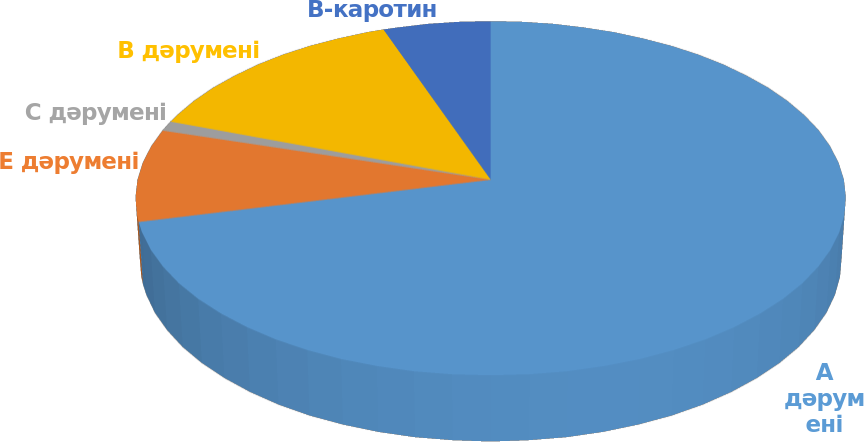
\includegraphics[width=0.65\textwidth]{media/pish2/image27}
	\caption*{2 - сурет. Асқабақ қабығы мен дәнімен байытылған тұтас дәнді бидай ұнынан жасалған қытырлақ нанның (хлебцы) құрамындағы дәрумендер мөлшері, г/100г.}
\end{figure}

\begin{multicols}{2}
Сонымен қатар, В тобындағы дәрумендер энергия деңгейін көтеріп, ағзаның
метаболизмін қолдайды. Бұл кестеде асқабақ қабығы мен дәнімен байытылған
тұтас дәнді бидай ұнынан жасалған қытырлақ нанның құрамындағы В
тобындағы дәрумендердің мөлшері берілген. Әр дәруменнің нақты алынған
көрсеткіші және оған сәйкес сынау әдістемесінің нормативтік құжаты (НҚ)
көрсетілген. Асқабақ қабығы мен дәнімен байытылған тұтас дәнді бидай
ұнынан жасалған қытырлақ нанның құрамындағы В тобындағы дәрумендер
мөлшері 2 - кестеде көрсетілген.
\end{multicols}

\begin{table}[H]
\caption*{2 - кесте. Асқабақ қабығы мен дәнімен байытылған тұтас дәнді бидай ұнынан жасалған қытырлақ нанның (хлебцы) құрамындағы В тобындағы дәрумендер мөлшері, г/100г.}
\centering
\begin{tblr}{
  row{1} = {c},
  column{2} = {c},
  hlines,
  vlines,
}
Көрсеткіш атауы      & Нақты алынған көрсеткіш & Сынау әдістемелерінің НҚ \\
В$_1$ дәрумені, мг/100г & 0,35±0,07               & ГОСТ 31483-2012          \\
В$_2$ дәрумені, мг/100г & 0,29±0,12               & ГОСТ 31483-2012          \\
В$_6$ дәрумені, мг/100г & 0,39±0,08               & ГОСТ 31483-2012          \\
В$_5$ дәрумені, мг/100г & 1,54±0,31               & ГОСТ 31483-2012          \\
В$_3$ дәрумені, мг/100г & 0,17±0,03               & ГОСТ 31483-2012          
\end{tblr}
\end{table}

\begin{figure}[H]
	\centering
	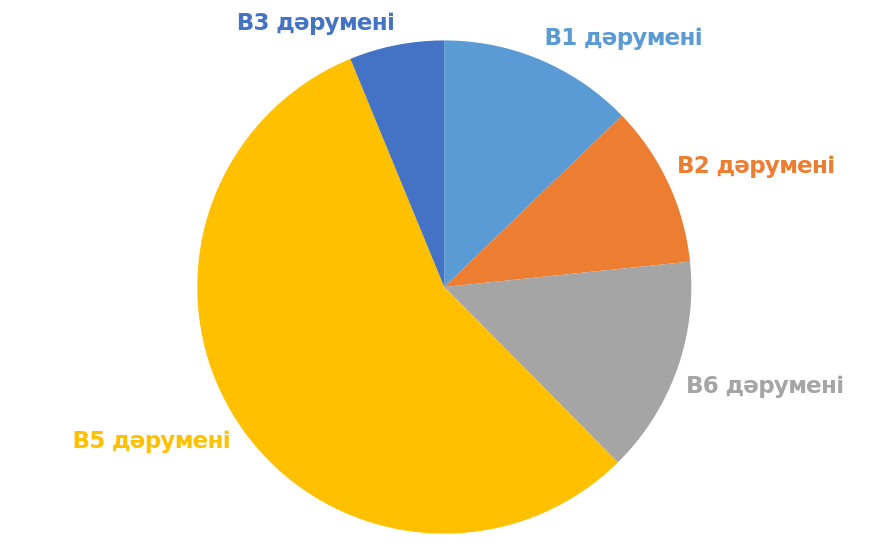
\includegraphics[width=0.65\textwidth]{media/pish2/image28}
	\caption*{3 - сурет. Асқабақ қабығы мен дәнімен байытылған тұтас дәнді бидай ұнынан жасалған қытырлақ нанның (хлебцы) құрамындағы В тобындағы дәрумендер мөлшері}
\end{figure}

\begin{multicols}{2}
В1 дәрумені 100 грамм өнімге шамамен 0,35мг көрсеткішке ие. В1 дәрумені
(тиамин) көмірсулар мен майлардың дұрыс метаболизмін қолдайды, жүйке
жүйесіне маңызды әсер етеді. Бұл көрсеткіш аздаған мөлшерде болғанымен,
оның жетіспеушілігі жүйке жүйесіне теріс әсер етуі мүмкін. Бірақ бұл
деңгейде В1 дәрумені жеткілікті деп айтуға болады. В2 дәрумені 100 грамм
өнімге шамамен 0,29 мг болды. В2 дәрумені (рибофлавин) энергия өндіруде
маңызды рөл атқарады және жасушалардың қалпына келуін қамтамасыз етеді.
Бұл мөлшердің қалыпты деңгейде болуы жақсы, бірақ оның көбірек болуы
ағза үшін зиянды емес. В6 дәрумені 100 грамм өнімде шамамен 0,39 мг
болды. В6 дәрумені (пиридоксин) ақуыздар мен майлардың метаболизміне
қатысады, сондай-ақ жүйке жүйесінің жұмысын қолдайды. Бұл деңгейде В6
дәруменінің мөлшері орташа, яғни ол денсаулық үшін пайдалы, бірақ басқа
көздермен толықтыруға болады. В5 дәрумені 100 грамм өнімде шамамен 1,54
мг болды. В5 дәрумені (пантотен қышқылы) энергияның өндірілуін қолдайды,
сондай-ақ стресс пен алаңдаушылықты азайтуға көмектеседі. Бұл мөлшер
қалыпты болып саналады, оның денсаулыққа пайдалы деңгейде. В3 дәрумені
100 грамм өнімде шамамен 0,17 мг болды{\bfseries .} В3 дәрумені (ниацин)
метаболизм процестеріне қатысады және теріні қорғауға көмектеседі. Оның
мөлшері төмен, бұл оның көп болмауын талап етпейтінін көрсетеді, бірақ
ол міндетті түрде басқа өнімдерден алынып отыруы тиіс. Асқабақ қабығы
мен дәнімен байытылған тұтас дәнді бидай ұнынан жасалған қытырлақ нанның
құрамындағы В тобындағы дәрумендер мөлшерін 3-суретте анық көре аламыз.

Өнімдер микробиологиялық тұрғыдан тексерілді. Тұтас дәнді бидай ұнынан
жасалған қытырлақ нанның (хлебцы), асқабақ қабығы мен дәнінде сапалы
микробиологиялық көрсеткіштер байқалды. Микробтар саны шекті деңгейде
болды, бұл асқабақ пен бүтін бидай ұнының микробқа қарсы қасиеттерін
және өңдеудегі санитарлық жағдайдың жақсы ұйымдастырылғанын көрсетеді.
Зерттеу нәтижелерін төменде көрсетілген 3-кестеде анық көре аламыз.
\end{multicols}

\begin{table}[H]
\caption*{3 - кесте. Асқабақ қабығы мен дәнімен байытылған тұтас дәнді бидай ұнынан жасалған қытырлақ нанның (хлебцы) құрамындағы микробиологиялық көрсеткіштері, г/100г.}
\centering
\begin{tblr}{
  colspec = {X[1.5] X[1] X[1] X[1]},
  cell{2}{2} = {c},
  cell{2}{3} = {c},
  cell{3}{2} = {c},
  cell{3}{3} = {c},
  cell{4}{2} = {c},
  cell{4}{3} = {c},
  hlines,
  vlines,
}
Көрсеткіш атауы                                  & НҚ бойынша рұқсат етілетін норма & Нақты алынған көрсеткіш & Сынау әдістемелерінің НҚ \\
КМАФАнМ, КОЕ/г, көп емес                         & 1х10\textsuperscript{3}          & 6х10\textsuperscript{2} & ГОСТ 10444.15-94         \\
БГКП, (колиформы) 1,0 см\textsuperscript{3} өнім & рұқсат етілмейді                 & анықталмады             & ГОСТ 31747-2012          \\
Плесень, КОЕ/г, көп емес                         & 50                               & 7                       & ГОСТ 10444.12-2013       
\end{tblr}
\end{table}

\begin{multicols}{2}
КМАФАнМ (Көп мөлшердегі мезофильді аэробты микроорганизмдер) - КОЕ/г,
нормативті құжат бойынша рұқсат етілген норма 1х10³ КОЕ/г аспау қажет.
Нақты алынған көрсеткіш 6х10² КОЕ/г болды. КМАФАнМ --- бұл өнімдегі
микроорганизмдер саны, негізінен, азық-түлік қауіпсіздігін бақылауға
арналған көрсеткіш. Мезофильді микроорганизмдер 20-45°C температурада
көбейетін микроорганизмдер. Бұл көрсеткіштің жоғары болуы өнімнің ұзақ
уақыт сақталуы мен сапасына әсер етуі мүмкін. Алайда, көрсеткіш 6х10²
КОЕ/г болғандықтан, бұл нормаға толықтай сәйкес келеді және өнімде
санитарлық талаптарға сай қауіпсіз деңгейде микроорганизмдер бар екенін
көрсетеді.

БГКП (Бауыр колиформа бактериялары) нормативті құжат бойынша рұқсат
етілмейді. Нақты алынған көрсеткіште анықталмады. БГКП (болса, көбінесе
Escherichia coli немесе басқа колиформа бактериялары) --- адамның ішек
флорасының бөлігі болғанымен, олардың тағамда болуы қауіпті, өйткені бұл
бактериялар патогенді болуы мүмкін және ауруларды таратуы ықтимал.
Колиформды бактериялардың өнімде болмауы керек, себебі оларды жұтқан
адам асқазан-ішек ауруларына ұшырауы мүмкін. Кестедегі нәтиже ---
"анықталмады", яғни бұл бактериялар өнімде жоқ, сондықтан бұл өте жақсы
көрсеткіш.

Плесень - КОЕ/г нормативті құжат бойынша рұқсат етілген норма 50 КОЕ/г.
Нақты алынған көрсеткіш 7 КОЕ/г көрсетті. Плесень --- бұл
саңырауқұлақтардың кейбір түрлері, олардың өсуі өнімнің сапасына әсер
етуі мүмкін. Плесеньнің көп болуы өнімнің құндылығын төмендетеді,
тағамның бұзылуына және дәмі мен хош иісінің нашарлауына әкеледі. Норма
бойынша бұл көрсеткіш 50 КОЕ/г аспауы керек. Ал нақты көрсеткіш 7 КОЕ/г
болғанда, бұл өте төмен және тағамның сапасы мен қауіпсіздігі жақсы
екенін көрсетеді.

Микробиологиялық талдау нәтижелері көрсеткендей, асқабақтың қабығы мен
дәнінде, сондай-ақ бүтін бидай ұнынан жасалған хлебцыде микробиологиялық
сапасы жоғары болды. Бұл өнімдерде патогенді микроорганизмдердің жоқтығы
немесе минималды болуы олардың азық-түлік қауіпсіздігі үшін маңызды
екенін көрсетеді. Мұндай нәтижелер өнімдердің жоғары сапасын және дұрыс
өңдеу процестерін растайды.

{\bfseries Қорытынды} Бұл зерттеу асқабақ қабығы мен асқабақ дәнімен
байытылған тұтас дәнді бидай ұнынан жасалған қытырлақ нанның (хлебцы)
қоректік құндылығы мен микробиологиялық көрсеткіштерін зерттеу
мақсатында жүргізілді. Асқабақ және тқтас дәнді бидай ұнының тағамдық
құндылығы жоғары, себебі олар көптеген дәрумендер (A, C, E, B тобы),
минералдар және басқа да биологиялық белсенді қосылыстарға бай. Атап
айтқанда, асқабақ дәндері мен қабығының құрамындағы витаминдер мен
минералдар тағамды ағза үшін пайдалы етеді.

Зерттеу нәтижелері қытырлақ нанның көптеген маңызды дәрумендер мен
микроэлементтердің болғанын көрсетті, сонымен қатар бұл өнімдердің
микробиологиялық қауіпсіздігі де маңызды болып табылды. КМАФАнМ, БГКП
және плесеньдер сияқты микроорганизмдердің анықталуы өнімнің сапасын
және оның сақталу мерзімін бақылауға мүмкіндік береді. Әрбір
микроорганизмнің санын анықтау және оларды бақылау тағам өнімдерінің
сапасын қамтамасыз етуге мүмкіндік береді.

Зерттеу барысында қолданылған микробиологиялық әдістер, соның ішінде
жоғары сұйықтықты хроматография (HPLC) әдісі дәрумендер мен
микроорганизмдердің концентрациясын дәл анықтауға мүмкіндік берді.
Нәтижесінде, асқабақ және тұтас дәнді бидай ұнынан жасалған хлебцыдің
қоректік құндылығы мен қауіпсіздігі жоғары деңгейде екені дәлелденді.

Асқабақ қабығы мен дәнімен байытылған тұтас дәнді бидай ұнынан жасалған
қытырлақ нанның құрамында витаминдер көбінесе жеткілікті деңгейде және
пайдалы. А дәрумені мен Е дәруменінің мөлшері жоғары, бұл өнімді
иммундық жүйені қолдау және антиоксиданттық қасиеттерді жақсарту үшін
жақсы таңдау етеді. Бірақ С дәрумені мен В3 дәруменінің мөлшері төмен
болуы мүмкін, сондықтан олардың жетіспеушілігін толтыру үшін басқа
көкөністер мен жемістерді тұтыну ұсынылады.

Барлық көрсеткіштер бойынша өнім санитарлық нормаларға сәйкес келеді.
Нақты алынған мәндер көрсеткендей, асқабақ қабығы мен дәнімен байытылған
тұтас дәнді бидай ұнынан жасалған қытырлақ нанның микробиологиялық
сапасы қауіпсіз әрі жақсы деңгейде сақталған. Әсіресе, БГКП (колиформды
бактериялар) болмауы, плесеньнің төмен деңгейі, және КМАФАнМ
көрсеткішінің нормадан асып кетпеуі өнімнің тазалығы мен денсаулыққа
қауіпсіз екенін білдіреді.

Қорытындылай келе, асқабақ қабығы мен дәнінен жасалған қытырлақ нан
(хлебцы) денсаулыққа пайдалы тағам ретінде ұсынылуы мүмкін. Бұл өнімнің
құрамындағы дәрумендер мен микроэлементтер ағзаға қажетті қоректік
заттарды қамтамасыз етеді, ал микробиологиялық көрсеткіштері оның
қауіпсіздігін және ұзақ уақыт бойы сақталуын қамтамасыз етеді. Аталған
зерттеу нәтижелері осы өнімдер өндірісінде қолданылатын технологияларды
әрі қарай жақсартуға және жаңа, пайдалы тағам өнімдерін жасауға үлес
қосады.
\end{multicols}

\begin{center}
{\bfseries Әдебиеттер}
\end{center}

\begin{references}
1.  Бижанова З.К., Алгазинова А.А., Садвакасова М.А., Алтайулы С. Разработка
технологии производства хлебобулочных изделий из композиции различных
видов зерновых культур // Материалы Республиканской научно-теоретической
конференции «Сейфуллинские чтения-12: Молодежь в науке -инновационный
потенциал будущего".-2016. -Т.1, ч.2. - С.22-26

2.  Байысбаева М.П. Наубайхана өндірісінде қолданылатын шикізаттар мен
материалдар. - Алматы: «Алейрон», 2009. - 93 б. ISBN 978-601-263-063-3

3.  Байысбаева М.П., Изембаева А.К., Жұманазар Д.Б., Молдақұлова З.Н., Тыным
Б.Қ. Зығыр дәнін хлебцы өнімінің рецептурасында қолдану// Алматы
технологиялық университетінің хабаршысы. -2023. -№2. -Б. 99-106. DOI
10.48184/2304-568X-2023-2-99-106

4.  Изембаева А.К., Байысбаева М.П., Молдақұлова З.Н., Байбатыров Т.А. Бүтін
тартылған ұндар қоспасынан дайындалған нан өнімінің сапасын бағалау //
Алматы технологиялық университетінің хабаршысы. - 2022.- №2. - Б. 67-73.
DOI 10.48184/2304-568X-2022-1-67-73.

5.  Батырбаева Н.Б., Рустемова А.Ж., Аскарбеков Э.Б. Дәнді-бұршақ қоспасынан
нан дайындау технологиясы // Алматы технологиялық университетінің
хабаршысы. -2022. - №2. -Б. 23-29. DOI \\10.48184/2304-568X-2022-1-23-29.

6.  Алашбаева Л.Ж., Боранкулова А.С., Турсунбаева Ш.А., Нургожина Ж.К.,
Баялы А.А. Функционалды бағыттағы нан өнімдерінің технологиясы //
Шәкәрім Университетінің Хабаршысы. Техникалық ғылымдар сериясы. -2024.-№
1(13). - Б. 81-89. DOI 10.53360/2788-7995-2024-1(13)

7.  Жумалиева Г.Е., Чоманов У.Ч., Актокалова Г.С., Идаятова М., Тултабаев
Н. Разработка технологии купажированных соков на основе тыквы
//Вестник АТУ. - 2023. -№1. - Б. 63-72. DOI\\
10.48184/2304-568X-2023-1-63-72.

8.  Икрами М.Б., Шарипова М.Б., Абдуллоева Х.Ф. Влияние некоторых факторов
на водоудерживающую и жироудерживающую способности тыквенной муки //
Вестник АТУ-2023. -№4.- Б.156-164. DOI
10.48184/2304-568X-2023-4-156-164

9.  Саидов А.М., Калитка Д.А., Молдахметова З.К., Екатеринская Е.М.,
Жангабылова Н.Д., Балгужинова Ж.Е. Тұтас дәнді ұн қосылған макарон
өнімдерінің рецептурасын әзірлеу // Алматы технологиялық
университетінің хабаршысы.- 2022.- №4.- Б.69-75. DOI
10.48184/2304-568X-2022-4-69-75.

10.  Sanjukta Kar, Suchandra Dutta, Rubina Yasmin, A comparative study on
phytochemicals and \\antioxidant activity of different parts of pumpkin
(Cucurbita maxima) // Food Chemistry Advances. -2023. -Vol. 3(5):100505.
DOI 10.1016/j.focha.2023.100505

11.  Aquino-Bolaños E.N., Urrutia-Hernández T.A., López Del Castillo-Lozano
M., Chavéz-Servia J.L., Verdalet-Guzmán I. Physicochemical Parameters
and Antioxidant Compounds in Edible Squash (Cucurbita pepo) Flower
Stored under Controlled Atmospheres // Journal of Food Quality.- 2013.
- Vol. 36(5). - P. 302--308. DOI 10.1111/jfq.12053.

12.  Vaher M., Matso K., Levandi T., Helmja K., Kaljurand M. Phenolic
compounds and the antioxidant activity of the bran, flour and whole
grain of different wheat varieties // Procedia Chemistry. -2010. -Vol.
2(1). - P.76-82. DOI 10.1016/j.proche.2009.12.013.

13.  Hussain A., Kausar T., Sehar S., Sarwar A., Ashraf A.H., Jamil M.A.,
Noreen S., Rafique A., Iftikhar K., Quddoos M.Y., Aslam J., Majeed
M.A. A Comprehensive review of functional ingredients, especially
bioactive compounds present in pumpkin peel, flesh and seeds, and
their health benefi//Fod Chemistry Advances.- 2022.-Vol.1(4):100067.
DOI 10.1016/j.focha.2022.100067.

14.  Szymczycha-Madeja A. Rapid method of element determination in rye
crispbread by ICP OES//Arabian Journal of Chemistry.- 2017. - Vol.
10(S2). - P. S3913--S3919.
DOI 10.1016/j.arabjc.2014.05.031.

15.  Dyshlyuk L., Babich O., Prosekov A., Ivanova S., Pavsky V., Yang Y. In
vivo study of medical and biological properties of functional bakery
products with the addition of pumpkin flour // Bioactive Carbohydrates
and Dietary Fiber.- 2017. -Vol. 2. -P. 20-24.
DOI 10.1016/j.bcdf.2017.09.001.

16.  Hagos M., Chandravanshi B., Redi-Abshiro M., Yaya E. E. Determination
of total phenolic, total flavonoid, ascorbic acid contents and
antioxidant activity of pumpkin flesh, peel and seeds // The Bulletin
of the Chemical Society of Ethiopia.- 2023. - Vol. 37(5). - P.
1093-1108.
DOI 10.4314/bcse.v37i5.3.

17.  Hagos M., Redi-Abshiro M., Chandravanshi B. S., Yaya E. E. Development
of analytical methods for determination of β-carotene in pumpkin
(Cucurbita maxima) flesh, peel, and seed powder samples //
International Journal of Analytical Chemistry. -2022. -Vol.
2022:9363692.
DOI 10.1155/2022/9363692.

18.  R.N. Sofia, S. Pernilla, N. Susanne, et al., Green color drives
rejection of crackers added with algae in children but not in adults
// Food Quality and Preference. -2025. -Vol 127(4): 105461
DOI \\10.1016/j.foodqual.2025.105461

19.  Lorena Gonzґalez-Gґomez, Gema Casado-Hidalgo, Damiґan
Pґerez-Quintanilla, Sonia Morante-\\Zarcero, Isabel Sierra. Evaluating
the stability of tropane and opium alkaloids during baking in homemade
gluten-free poppy seed crackers // LWT - Food Science and Technology.
-2024. --Vol. 214. DOI\\
\href{https://doi.org/10.1016/j.lwt.2024.117080}{10.1016/j.lwt.2024.117080}
\end{references}

\begin{center}
{\bfseries References}
\end{center}

\begin{references}
1. Bizhanova Z.K., Algazinova A.A., Sadvakasova M.A., Altajuly S.
Razrabotka tehnologii proizvodstva hlebobulochnyh izdelij iz kompozicii
razlichnyh vidov zernovyh kul' tur // Materialy
Respublikanskoj nauchno-teoreticheskoj konferencii «Sejfullinskie
chtenija-12: Molodezh'{} v nauke -innovacionnyj \\potencial
budushhego".-2016. -T.1, ch.2. - S.22-26. {[}in Russian{]}

2. Bajysbaeva M.P. Naubajhana өndіrіsіnde қoldanylatyn shikіzattar men
materialdar. - Almaty: «Alejron», 2009. - 93 b. ISBN 978-601-263-063-3.
{[}in Kazakh{]}

3. Bajysbaeva M.P., Izembaeva A.K., Zhұmanazar D.B., Moldaқұlova Z.N.,
Tynym B.Қ. Zyғyr dәnіn hlebcy өnіmіnің recepturasynda қoldanu// Almaty
tehnologijalyқ universitetіnің habarshysy. -2023. -№2. -B. 99-106. DOI
10.48184/2304-568X-2023-2-99-106. {[}in Kazakh{]}

4. Izembaeva A.K., Bajysbaeva M.P., Moldaқұlova Z.N., Bajbatyrov T.A.
Bүtіn tartylғan ұndar қospasynan dajyndalғan nan өnіmіnің sapasyn
baғalau // Almaty tehnologijalyқ universitetіnің habarshysy. - 2022.-
№2. - B. 67-73. DOI 10.48184/2304-568X-2022-1-67-73. {[}in Kazakh{]}

5. Batyrbaeva N.B., Rustemova A.Zh., Askarbekov Je.B. Dәndі-bұrshaқ
қospasynan nan dajyndau \\tehnologijasy // Almaty tehnologijalyқ
universitetіnің habarshysy. -2022. - №2. -B. 23-29. DOI\\
10.48184/2304-568X-2022-1-23-29. {[}in Kazakh{]}

6. Alashbaeva L.Zh., Borankulova A.S., Tursunbaeva Sh.A., Nurgozhina
Zh.K., Bajaly A.A. Funkcionaldy baғyttaғy nan өnіmderіnің tehnologijasy
// Shәkәrіm Universitetіnің Habarshysy. Tehnikalyқ ғylymdar serijasy.
-2024.-№ 1(13). - B. 81-89. DOI 10.53360/2788-7995-2024-1(13). {[}in
Kazakh{]}

7. Zhumalieva G.E., Chomanov U.Ch., Aktokalova G.S., Idajatova M.,
Tultabaev N. Razrabotka tehnologii kupazhirovannyh sokov na osnove tykvy
//Vestnik ATU. - 2023. -№1. - B. 63-72. DOI
10.48184/2304-568X-2023-1-63-72. {[}in Russian{]}

8. Ikrami M.B., Sharipova M.B., Abdulloeva H.F. Vlijanie nekotoryh
faktorov na vodouderzhivajushhuju i zhirouderzhivajushhuju sposobnosti
tykvennoj muki // Vestnik ATU-2023. -№4.- B.156-164. DOI\\
10.48184/2304-568X-2023-4-156-164. {[}in Russian{]}

9. Saidov A.M., Kalitka D.A., Moldahmetova Z.K., Ekaterinskaja E.M.,
Zhangabylova N.D., Balguzhinova Zh.E. Tұtas dәndі ұn қosylғan makaron
өnіmderіnің recepturasyn әzіrleu // Almaty tehnologijalyқ\\
universitetіnің habarshysy.- 2022.- №4.- B.69-75. DOI
10.48184/2304-568X-2022-4-69-75. {[}in Kazakh{]}

10. Sanjukta Kar, Suchandra Dutta, Rubina Yasmin, A comparative study on
phytochemicals and \\antioxidant activity of different parts of pumpkin
(Cucurbita maxima) // Food Chemistry Advances. -2023. -Vol. 3(5):100505.
DOI 10.1016/j.focha.2023.100505

11. Aquino-Bolaños E.N., Urrutia-Hernández T.A., López Del
Castillo-Lozano M., Chavéz-Servia J.L., Verdalet-Guzmán I.
Physicochemical Parameters and Antioxidant Compounds in Edible Squash
(Cucurbita pepo) Flower Stored under Controlled Atmospheres // Journal
of Food Quality.- 2013. - Vol. 36(5). - P. 302--308. DOI
10.1111/jfq.12053.

12. Vaher M., Matso K., Levandi T., Helmja K., Kaljurand M. Phenolic
compounds and the antioxidant activity of the bran, flour and whole
grain of different wheat varieties // Procedia Chemistry. -2010. -Vol.
2(1). - P.76-82. DOI 10.1016/j.proche.2009.12.013.

13. Hussain A., Kausar T., Sehar S., Sarwar A., Ashraf A.H., Jamil M.A.,
Noreen S., Rafique A., Iftikhar K., Quddoos M.Y., Aslam J., Majeed M.A.
A Comprehensive review of functional ingredients, especially bioactive
compounds present in pumpkin peel, flesh and seeds, and their health
benefi//Fod Chemistry Advances.- 2022.-Vol.1(4):100067.
DOI 10.1016/j.focha.2022.100067.

14. Szymczycha-Madeja A. Rapid method of element determination in rye
crispbread by ICP OES//Arabian Journal of Chemistry.- 2017. - Vol.
10(S2). - P. S3913--S3919. DOI 10.1016/j.arabjc.2014.05.031.

15. Dyshlyuk L., Babich O., Prosekov A., Ivanova S., Pavsky V., Yang Y.
In vivo study of medical and biological properties of functional bakery
products with the addition of pumpkin flour // Bioactive Carbohydrates
and Dietary Fiber.- 2017. -Vol. 2. -P. 20-24.
DOI 10.1016/j.bcdf.2017.09.001.

16. Hagos M., Chandravanshi B., Redi-Abshiro M., Yaya E. E. Determination
of total phenolic, total flavonoid, ascorbic acid contents and
antioxidant activity of pumpkin flesh, peel and seeds // The Bulletin of
the Chemical Society of Ethiopia.- 2023. - Vol. 37(5). - P. 1093-1108.
DOI 10.4314/bcse.v37i5.3.

17. Hagos M., Redi-Abshiro M., Chandravanshi B. S., Yaya E. E.
Development of analytical methods for determination of β-carotene in
pumpkin (Cucurbita maxima) flesh, peel, and seed powder samples //
International Journal of Analytical Chemistry. -2022. -Vol.
2022:9363692. DOI 10.1155/2022/9363692.

18. R.N. Sofia, S. Pernilla, N. Susanne, et al., Green color drives
rejection of crackers added with algae in children but not in adults //
Food Quality and Preference. -2025. -Vol 127(4): 105461
DOI \\10.1016/j.foodqual.2025.105461

19. Lorena Gonzґalez-Gґomez, Gema Casado-Hidalgo, Damiґan
Pґerez-Quintanilla, Sonia Morante-\\Zarcero, Isabel Sierra. Evaluating the
stability of tropane and opium alkaloids during baking in homemade
gluten-free poppy seed crackers // LWT - Food Science and Technology.
-2024. -Vol. 214. DOI\\
\href{https://doi.org/10.1016/j.lwt.2024.117080}{10.1016/j.lwt.2024.117080}
\end{references}

\begin{authorinfo}
\emph{{\bfseries Авторлар туралы мәліметтер}}

Алибаева Д.Қ. - техника ғылымдарының магистрі, докторант, Мұхтар Ауезов
атындағы Оңтүстік Қазақстан Университетіі, Шымкент, Қазақстан, e-mail:
\href{mailto:dinaalibayeva3@gmail.com}{\nolinkurl{dinaalibayeva3@gmail.com}};

Иманбаев А.Ж. - техника ғылымдарының кандидаты, доцент, Мұхтар Ауезов
атындағы Оңтүстік Қазақстан Университеті, Шымкент, Қазақстан, e-mail:
\href{mailto:Algo79@mail.ru}{\nolinkurl{Algo79@mail.ru}};

Hülya Gül - Professor, Süleyman Demirel University, Faculty of
Engineering and Natural Sciences, Department of Food Engineering,
Isparta, Türkiye, е-mail:
\href{mailto:hulyagul@sdu.edu.tr}{\nolinkurl{hulyagul@sdu.edu.tr}};

Есиркеп Г.Е.- техника ғылымдарың кандидаты, қауымдастырылған профессор,
Қ.Құлажанов атындағы Қазақ технология және бизнес университеті, Астана,
Қазақстан, e-mail:
\href{mailto:milana.anar@mail.ru}{\nolinkurl{milana.anar@mail.ru}};

Нармандах Ж. - магистр, ассистент, Қ. Құлажанов атындағы Қазақ
технология және бизнес университеті, Астана, Қазақстан, e-mail:
\href{mailto:zhupar10_89@mail.ru}{\nolinkurl{zhupar10\_89@mail.ru}};

\emph{{\bfseries Information about the authors}}

Alibayeva D.K.- Master of Technical Sciences, PhD student, M. Auezov
South Kazakhstan University, Shymkent, Kazakhstan, е-mail:
\href{mailto:dinaalibayeva3@gmail.com}{\nolinkurl{dinaalibayeva3@gmail.com}};

Imanbayev A.Zh.- Candidate of Technical Sciences, Docent, M. Auezov
South Kazakhstan University, Shymkent, Kazakhstan, е -mail:
\href{mailto:Algo79@mail.ru}{\nolinkurl{Algo79@mail.ru}};

Hülya Gül -- Professor, Süleyman Demirel University, Faculty of
Engineering and Natural Sciences, Department of Food Engineering,
Isparta, Türkiye, е-mail:
\href{mailto:hulyagul@sdu.edu.tr}{\nolinkurl{hulyagul@sdu.edu.tr}};

Yesirkep G. Y.-Candidate of Technical Sciences, Associate Professor,
Kazakh University of Technology and Business named after K. Kulazhanov,
Astana, Kazakhstan, e-mail:
\href{mailto:milana.anar@mail.ru}{\nolinkurl{milana.anar@mail.ru}};

Narmandakh Zh. - Master's Degree, Assistant, Kazakh University of
Technology and Business named after K. Kulazhanov, Astana, Kazakhstan,
e-mail: zhupar10\_89@mail.ru.
\end{authorinfo}
